\documentclass[10pt]{paper}

\usepackage{minted}
\usepackage{amsmath}
\usepackage{latexsym}
\usepackage{float}
\usepackage{amssymb}
\usepackage{geometry}
\usepackage{graphicx}

\title{3 Questions}
\author{Timothy Schwieg}

\begin{document}

\maketitle
\section{How much does a Volvo V60 Cost?}

Consider an agent who is trying to determine how much a Volvo v60
costs. He must take into account the cost of the car, whether or not
he is taking out a loan, the maintenance that the car requires, as well
as repairs, insurance, fuel and registration. Since many of these
payments are made in the future, they will time discounted. Besides
these explicit costs, there is also the implicit cost of not investing
the money at some prevailing interest rate.

The Buyer faces some upfront prices: Down payment size, insurance
level, warranty.

In each time period the buyer must pay a loan payment, insurance, fuel
costs, registration, maintenance and repairs. Since insurance is
mandatory, we will claim insurance is actuarilly fair, so the choice
of insurance is irrelevant. We will take the minimum insurance package
as a result as it is easiest computationally. 

The buyer wishes to minimize the present value of these effects, using
geometric time discounting to figure out the cost of the Volvo V60.

We will consider loan payments to be monthly,
while maintenance, repairs, registration, insurance, and fuel costs to be yearly
payments. Time will be discounted by $\beta$ which is the discount per
month.

The amount of time the buyer spends driving will be taken as
exogenous, as the driver is purchasing the car for some task,
hopefully driving.

\subsection*{Setup}
%15k miles per year
\begin{align*}
  \min_{DP} \mathbb{E} DP  + \sum_{t=0}^T \beta^t (P) +
  \sum_{y=0}^Y \beta^{12y}(I + F_y (M_y + Rep_y) + Reg_y )\\
  P = \frac{r( MSRP - DP )}{1- (1+r)^{-T}}\\
  \beta = \frac{1}{1+r}\\ 
\end{align*}
$M_y, Rep_y$  are a sequence of maintence and repair costs.
$Reg_y$ is the cost of registering the vehicle yearly.
$F_y$ is the cost of gasoline in time period y, MSRP is the cost of
the Car, r is the prevailing interest rate.

\begin{align*}
  MSRP = 36150\\
  M_Y + Rep_y = 229\\
  F_t = \frac{15000}{12}*25*C_g(t)\\
  C_g = 2.607
\end{align*}

\subsection*{Code}
\begin{minted}[mathescape, fontsize=\small, xleftmargin=0.5em]{julia}
using JuMP
using SCIP
m = Model(solver=SCIPSolver())

MSRP = 36150
Main = 229
Fuel = 15000*25*2.607/12
r = 0.07/12.0
beta = 1/(1+r)
T = 36
Y = 10
I = 227
Reg_initial = 225
Reg = 72.40

@variable( m, 0<=D<=MSRP)
@expression( m, P, (r*(MSRP-D))/ (1-(1+r)^(-T) ) )
@objective(m, Min, Reg_initial +  sum( beta^i *(P+I) for i = 1:T ) + sum( beta^(12*i) * ( Fuel + Main + Reg ) for i =1:Y )  )
status = solve(m)
\end{minted}
\begin{minted}[fontsize=\small, xleftmargin=0.5em, mathescape, frame = leftline]{text}
feasible solution found by trivial heuristic after 0.0 seconds, objective v
alue -3.615000e+04
presolving:
presolving (1 rounds: 1 fast, 0 medium, 0 exhaustive):
 1 deleted vars, 0 deleted constraints, 0 added constraints, 0 tightened bo
unds, 0 added holes, 0 changed sides, 0 changed coefficients
 0 implications, 0 cliques
transformed 1/3 original solutions to the transformed problem space
Presolving Time: 0.00

SCIP Status        : problem is solved [optimal solution found]
Solving Time (sec) : 0.00
Solving Nodes      : 0
Primal Bound       : -3.61499999999998e+04 (3 solutions)
Dual Bound         : -3.61499999999998e+04
Gap                : 0.00 %
\end{minted}

\begin{minted}[mathescape, fontsize=\small, xleftmargin=0.5em]{julia}

println("Objective value: ", getobjectivevalue(m))
\end{minted}
\begin{minted}[fontsize=\small, xleftmargin=0.5em, mathescape, frame = leftline]{text}
Objective value: 575865.3235946147
\end{minted}



\section{How Much Should I save?}

We will consider this problem in the context of an LQ-control problem
of finding the optimal consumption path when facing some income.

We are considering a household budget of:
\begin{align*}
  a_{t+1} + c_t = (1+r)a_t + y_t\\
\end{align*}
We consider $a_t$ to be savings at time t, and $c_t$ to be
consumption, and $y_t$ to be non-financial income, or income earned by
working. We would like $y_t$ to be random, following some linear law
of motion. For simplicity let: $y_t \sim N( \mu , \sigma^2 ) $. We shall also
represent consumption as deviation from some ideal level of
consumption. That is we choose $u_t := c_t - \bar{c}$. Our budget
equation now becomes:
$$a_{t+1} = (1+r)a_t - u_t - \bar{c} + \sigma w_{t+1} + \mu $$
where $w_{t+1} = N(0,1)$ We wish to represent this in a linear State
space model, however we currently have an affline function, so we must
add a fake variable to allow for the model to be written as:
$$x_{t+1} = Ax_t + Bu_t + Cw_{t+1}$$
We shall define
$$x_t :=
\begin{bmatrix}
  a_t\\
  1\\
\end{bmatrix}
A :=
\begin{bmatrix}
  1+r & -\bar{c} + \mu\\
  0 & 1
\end{bmatrix}
 B :=
 \begin{bmatrix}
   -1\\
   0
 \end{bmatrix}
 C :=
 \begin{bmatrix}
   \sigma\\
   0
 \end{bmatrix}
$$

\subsection*{Preferences}

We wish to represent preferences as trying to minimize deviations of
the consumer from the optimal level of consumption. In fitting with
the LQ control model, we wish to minimize $u_t 1 u_t = u_t^2 =
(c_t - \bar{c})^2$ Since the LQ objective function is $x_t^T R x_t +
u_t^T Q u_t$ we shall set $R = \begin{bmatrix} 0 & 0 \\ 0 & 0 \end{bmatrix}$ and $Q = 1$. 

\subsection*{The Objective}

We wish to maximize time discounted consumption in each period with an
incentive to be debt-free at the end of life, as otherwise the
consumer would simply rack up endless debt to pay for optimal
consumption. We shall achieve this by defining the objective in the
final time period as: $R_f = \begin{bmatrix} q & 0\\ 0 &
  0 \end{bmatrix}$. Where q is suitably large enough. Our objective
function then is:
$$\min_{{\{c_t\}}_{t=0}^T}\mathbb{E} \sum_{t=0}^{T-1}\beta^t(c_t - \bar{c})^2
+ \beta^T q a_t^2$$


\subsection*{Further Investigation}
It is pretty unrealistic to assume income
doesn't change over time. We would like to consider parabolic income
where $y_t = m_0 + m_1t + m_2t^2 + \sigma w_{t+1}$ We will choose the m
values to determine the peek of income. Income begins at 0, rises to
$\mu$ at some point in his life, and falls to 0 again somewhere later
outside the ``end'' of his life. We will believe that the peak of the
agent's career occurs two thirds of the way through his life. That is:
$\frac{m_1}{2m_0} = \frac{2}{3}T$ and the roots of the parabola occur
at: 0, $\frac{4}{3}T$. This yields: $m_0 = 0, m_1 = 3\mu, m_2 =
\frac{-9\mu}{4}$.

Our income model has become slightly less fun:

$$a_{t+1} = (1+r)a_t - u_t - \bar{c} + \frac{3\mu t}{K} - \frac{9\mu}{4K^2}t^2 + \sigma
w_{t+1}$$
Our states have become:

$$x_t =
\begin{bmatrix}
  a_t\\1\\t\\t^2
\end{bmatrix}
A =
\begin{bmatrix}
  1+r & -\bar{c} & \frac{3 \mu}{K} & \frac{9\mu}{4K^2}\\
  0 & 1 & 0 & 0\\
  0 & 1 & 0 & 0\\
  0 & 1 & 2 & 1\\
\end{bmatrix}
 B =
 \begin{bmatrix}
   -1\\0\\0\\0
 \end{bmatrix}
C =
\begin{bmatrix}
  \sigma\\0\\0\\0
\end{bmatrix}
$$

Q,R,$R_f$ remain unchanged except for the increase in size.

\subsection*{Retirement}

Naturally, we only care about savings in order to figure out how much
we should save for retirement. This means our model cannot have the
lifetime of our agent ending before retirement. Our model simply
creates an incentive of being debt-free at the time of retirement, which doesn't
really make a lot of sense in the context of saving for retirement. We
wish to extend the lifetime infinitely in retirement where his income
is fixed but at a smaller amount than he could earn by
working. Hopefully this will incentives the agent to save money so
that he can still consume at a level he is used to in retirement.

This introduces a kink into our income formula.
\begin{align*}
  y = \begin{cases}
    m_0 + m_1t + m_2t^2 + \sigma w_{t+1}& \text{ if } t \leq K\\
    s & \text{ otherwise}\\
    \end{cases}
\end{align*}
To solve this problem, we will solve the infinite dynamic program,
finding the value function at the start of this program, and this will
become the value function at the end of the finite LQ program. This
means that we will be solving an infinite LQ Control problem in order
to figure out $R_f$ to determine the savings path.

\subsection*{Solving the Model}

\subsubsection*{Infinite Horizon}

We seek the solution to the LQ-Bellman equation given by:
$$P=R−(β B^T P A )^T (Q + β B^T P B)^{-1} (βB^T P A ) + βA^T P A$$
Our optimal policy will be given by:
$$u = -F x \text{ where } F = (Q + \beta B^T
P B )^{-1} ( \beta B^T P A)$$
Our optimal savings policy is then given by:
$$x_{t+1} = (A-BF)x_t + Cw_{t+1}$$
This P, the stationary distribution will be passed to the
Discrete interval question as the final state, allowing us to account
for the discontinuity in the income process.


\subsection*{Code}

\begin{minted}[mathescape, fontsize=\small, xleftmargin=0.5em]{julia}
using QuantEcon
using Plots
using Plots.PlotMeasures
pyplot()

r = 0.05
#This had to be a lot lower than expected to not get massive debt.
#I think this is because there is no incentive to be debt-free at the end of life.
#The current Linear State space cannot accomodate Only punishing negative $a_t$ so
#I am not sure how this could be worked around without provididing a completely different model
deathParam = 0.004
beta = 1/(1+r+deathParam)
T = 70
c_bar = 10.0
sigma = .5
mu = 5.0
s = 1
K = 45
q = 1e6
m1 = 3*mu/(K)
m2 = -9*mu/(4*(K)^2)

# == Formulate as an LQ problem == #
Q = 1.0
R = zeros(4, 4)



Rf = zeros(4, 4);
Rf[1, 1] = q
A = [1+r  s-c_bar 0 0;
     0     1      0 0;
     0     1      1 0;
     0     1      2 1]
B = [-1.0; 0.0; 0.0; 0.0]
C = [0.0; 0.0; 0.0; 0.0]

#Seek out the stationary distribution of the infinite LQ
lq_retired = LQ( Q, R, A, B, C, bet=beta)
stationary_values!( lq_retired )


Rf2 = lq_retired.P
beta = 1/(1+r)
Q = 1.0
R = zeros(4, 4)
A = [1 + r -c_bar m1 m2;
     0     1      0  0;
     0     1      1  0;
     0     1      2  1]
B = [-1.0; 0.0; 0.0; 0.0]
C = [sigma; 0.0; 0.0; 0.0]

# == Set up working life LQ instance with terminal Rf from lq_retired == #
lq_working = LQ(Q, R, A, B, C; bet = beta, capT = K, rf = Rf2)

# == Simulate working state / control paths == #
x0 = [0.0; 1.0; 0.0; 0.0]
xp_w, up_w, wp_w = compute_sequence(lq_working, x0)
# == Simulate retirement paths (note the initial condition) == #
xp_r, up_r, wp_r = compute_sequence(lq_retired, xp_w[:, end],T-K )

# == Convert results back to assets, consumption and income == #
xp = [xp_w xp_r[:, 2:end]]
assets = vec(xp[1, :])               # Assets

up = [up_w up_r]
c = vec(up + c_bar)                  # Consumption

time = 1:K
income_w = sigma * vec(wp_w[1, 2:K+1]) + m1 .* time + m2 .* time.^2   # Income
income_r = ones(T-K) * s
income = [income_w; income_r]

# == Plot results == #
p1 = plot(Vector[income, assets, c, zeros(T + 1)], lab = ["non-financial income" "assets" "consumption" ""],
     color = [:orange :blue :green :black], width = 3, xaxis = ("Time"), layout = (2,1),
          bottom_margin = 20mm, size = (600, 600), show = true)
\end{minted}
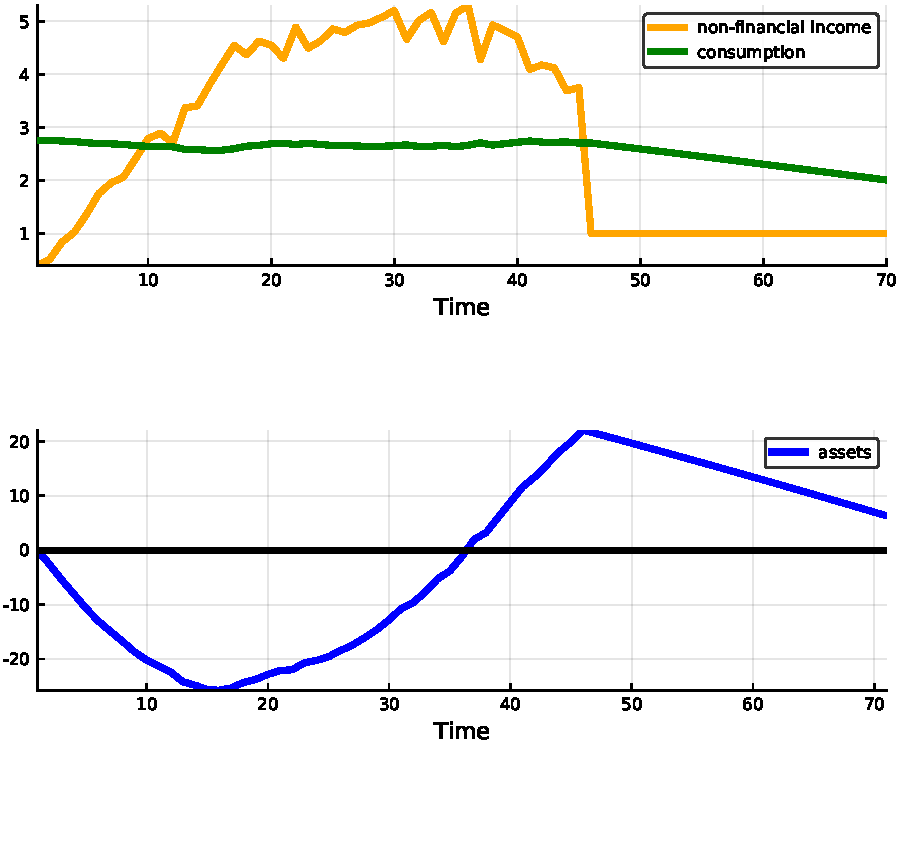
\includegraphics[width=\linewidth]{figures/questions_2_1.pdf}


This can be contrasted against the consumer who knows when the date he
will pass is. He is incentivised to be debt-free at the end of his life, and
knows the time when he will pass, he is able to leverage this into a
constant consumption level along his entire lifetime, while the
infinitely lived, but death discounting agent decreases his
consumption throughout retirement as he expects to die in the future,
and more highly values present consumption.


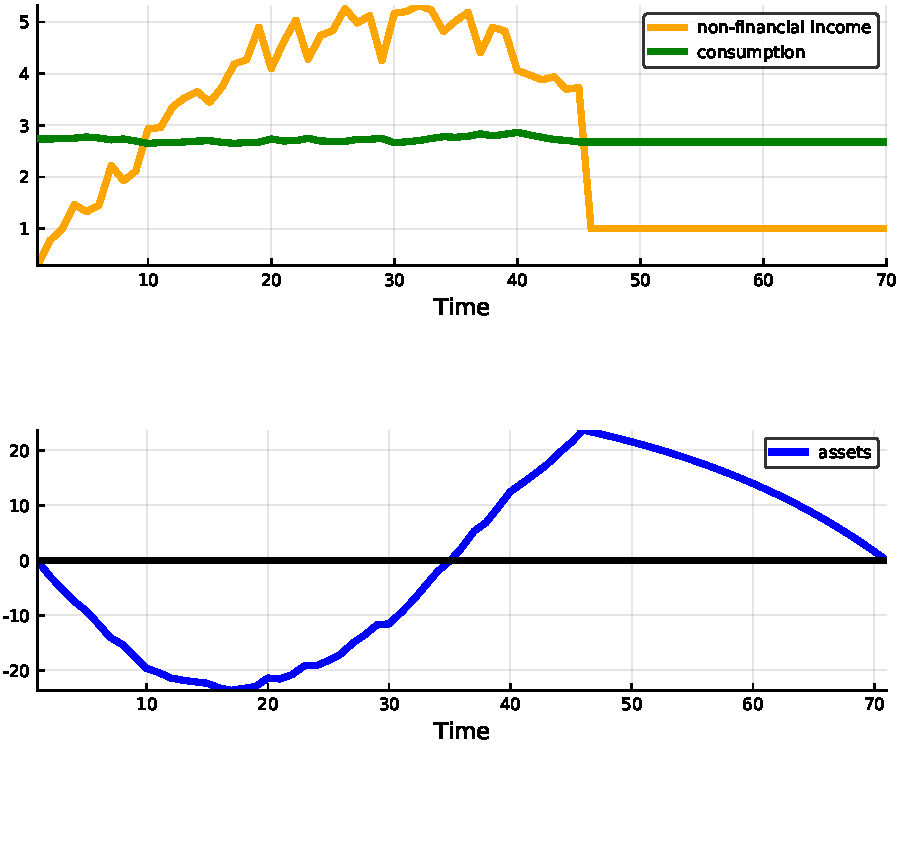
\includegraphics[width=\linewidth]{figures/questions_3_1.pdf}



We can see that the myopic consumer with the death wish consumes
higher in his lifetime, possibly leading to the death that he is so
certain of. The consumer who is uncertain of his death maintains his
savings so that he would be able to live off it indefinietly. One
explanation is he plans to pass on his wealth to his family, so
considering an infinite time horizen is legitimate. 

\section{Can I afford a House?}

\subsection*{The Problem}

I have chosen to consider that this question is asking whether or not
you should rent a house or buy one. I am taking the value of the house
as exogenous, as otherwise you could simply find a cheaper one and
this would be trivial.

By applying the Law of renting costs equals owning costs popularized
by the famous Economist Harry Paarsch in 2017, we can understand
that the costs of owning a house and renting should be relatively
close to each other. I will consider this arbitrage arguement true for
no down payment made on a house.

This condition leads us to a choice of down payment on a house, and if
we apply an income process that is increasing over the time of the
loan, we may choose optimal consumption over the lifetime of the agent
who pays payments on a loan for some fixed period of time, and always
pays maintenence fees on his house. The consumption under this model
may be compared to consumption under a model where the agent only pays
rent costs for his entire life. The question is whether or not there
is a down payment that is strictly better off in terms of consumption
over the renting option.

The arbitrage condition that this model rests upon is:
$$\mathbb{E}[\sum_{t=0}^\infty \beta^t C_R(t)] = \sum_{n=0}^N \beta^n P + \mathbb{E}[\sum_{t=0}^\infty
\beta^t C_m(t)$$
Where $C_R$ is the cost of renting, $C_m$ is the cost of maintaining
the house, P is the payments made on a house  and $\beta$ is some time
discounting factor.

We can simplify this by setting $C_R(t) = C_R$ and $C_m(t) = C_m$
Our arbitrage condition then simplifies to:
\begin{align*}
  \frac{C_R}{1-\beta} = P \frac{1-\beta^{N+1}}{1-\beta} + \frac{C_m}{1-\beta}\\
  C_R = P(1-\beta^{N+1}) + C_m\\
  C_R - C_m = P( 1- \beta^{N+1} )\\
  %P = \frac{r( V  )}{1- (1+r)^{-N}}\\
  %C_R - C_M= \frac{r V (1-\beta^{N+1})}{1- (1+r)^{-N}}
\end{align*}

\subsection*{Law of Motion}

We would like to follow the same law of motion as the savings problem,
where assets and consumption are equal to working and capital
income. We will seperate consumption from housing payments, and
consider the deviation of consumption from some ideal level as the
utility function.

\subsubsection*{Renter}
$$a_{t+1} = (1+r)a_t - u_t - \bar{c} + \frac{3\mu t}{K} - \frac{9\mu}{4K^2}t^2 + \sigma
w_{t+1} - C_R$$

$$x_t =
\begin{bmatrix}
  a_t\\1\\t\\t^2
\end{bmatrix}
A =
\begin{bmatrix}
  1+r & -\bar{c} - C_R & \frac{3 \mu}{K} & \frac{9\mu}{4K^2}\\
  0 & 1 & 0 & 0\\
  0 & 1 & 0 & 0\\
  0 & 1 & 2 & 1\\
\end{bmatrix}
 B =
 \begin{bmatrix}
   -1\\0\\0\\0
 \end{bmatrix}
C =
\begin{bmatrix}
  \sigma\\0\\0\\0
\end{bmatrix}
$$

This is effectively the same problem as before, as the renter simply has a lower
level of ideal consumption, or can be treated as having the same
amount of ideal consumption, but measurely less wealth in each
period.

\subsubsection*{Buyer}

The buyer however has a slightly different story: The buyer faces a
lower income for the periods in which he is paying off the hoouse, but
then has more income later in his life to enjoy. For the period in
which he is paying back his loans: $Y_R + P( 1- \beta^{N+1} ) - P = Y_R -
P \beta^{N+1}$
then changes after N periods to $Y_R + P( 1- \beta^{N+1} )$.

\subsection*{Code}


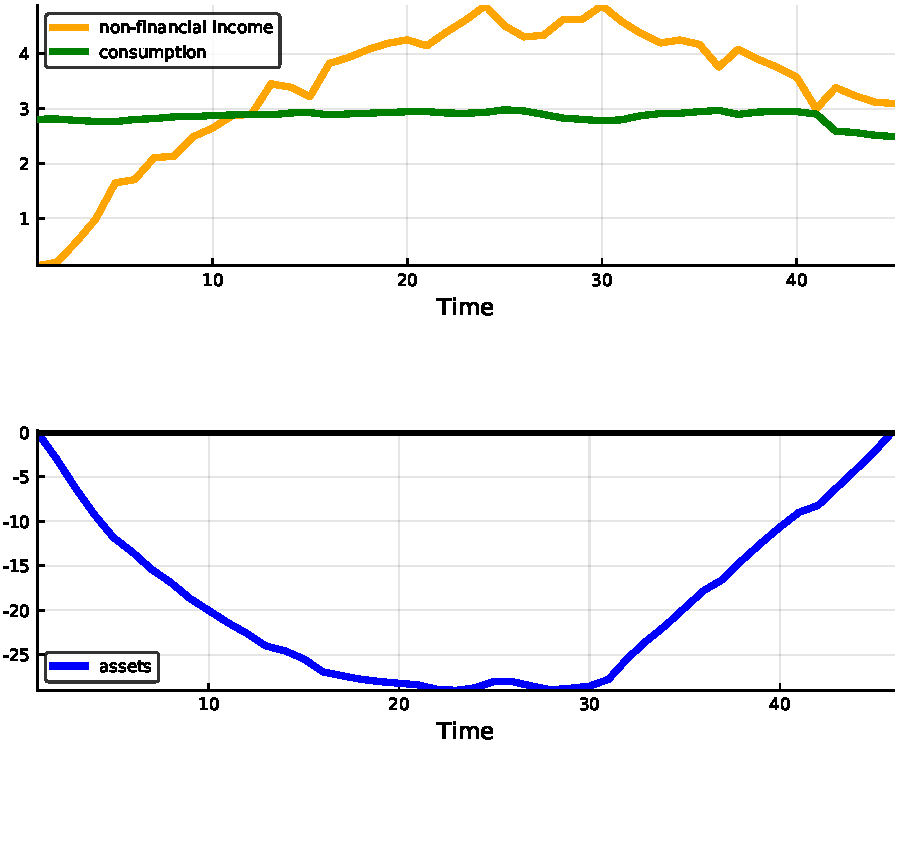
\includegraphics[width=\linewidth]{figures/questions_4_1.pdf}

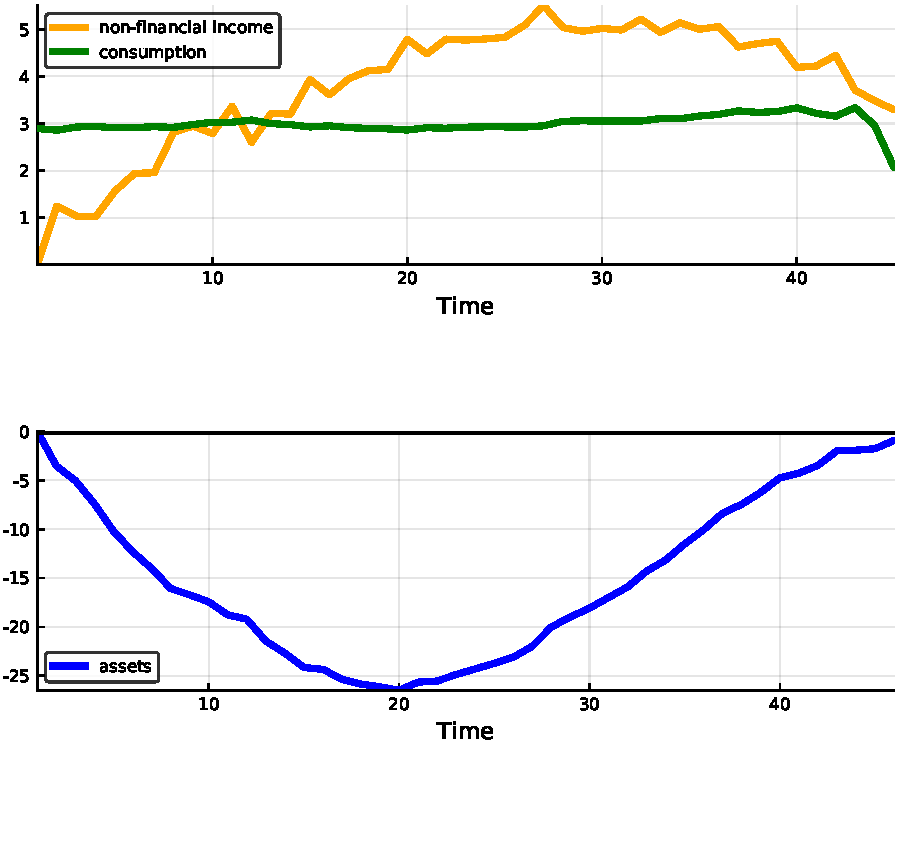
\includegraphics[width=\linewidth]{figures/questions_5_1.pdf}



We can see that under this arbitrage arguement, there is no reason to
buy a house over renting one of equal value. The Renter enjoys higher
consumption, and goes into less debt compared to the house
buyer. 


I am actually uncertain of how to properly cite my source here. But
almost everything I did with LQ control borrows very heavily from the
QuantEcon website by Thomas J. Sargent and John Stachurski. Their
section on LQ control from which all of my work is basically stolen
and then modified can be found at:
https://lectures.quantecon.org/jl/lqcontrol.html.


I attempted to keep their code as intact as possible when I made my
additions so that it could be followed easily, but if it would have
been better to not follow that please tell me so I don't plaigerize on
something much more important. 
\end{document}